\chapter{Grundlagen}

\section{Android}
\sectionauthor{\oliver}

\subsection{Activity}
Aktivitäten sind die Grundbausteine für eine Android-App. Sie dienen als 
Einstiegspunkt für die Interaktion des Benutzers der App. Hauptaufgaben einer 
\code{Activity} sind sowohl einen gelungenen Übergang zwischen dem Landscape und 
dem Portait Modus herzustellen, als auch dem System mitzuteilen, wann eine 
Prozess terminiert werden darf, ohne Benutzerinformationen zu verlieren. Für 
gewöhnlich füllt eine Aktivität einen kompletten Bildschirm aus, sie kann aber 
auch kleiner sein und über einer anderen \emph{schweben}. Typischerweise ist 
jeder Screen einer App eine eigene Activity, sodass eine Aktivität als 
\emph{main activity} spezifiziert wird, welche beim starten der App ausgeführt 
wird.

\subsection{Activity Lifecycle}
Der Activity Lifecycle beschreibt den Lebenszyklus einer Aktivität. Neben den 
drei Zuständen die eine Aktivität besitzt, beschreibt der Lifecycle auch die 
Methoden der Klasse \code{Activity}, welche nach belieben überschrieben werden 
können um bestimmte Statusübergänge zu programmieren.

\begin{figure}[h]
	\centering
	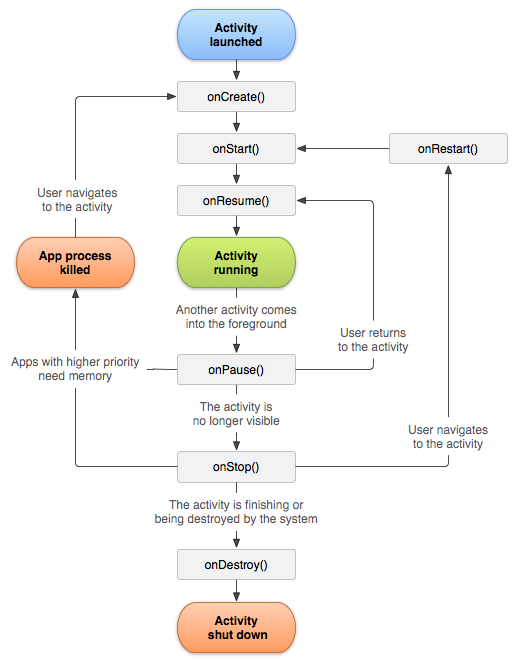
\includegraphics[width=0.5\textwidth]{resources/android/lifecycle}
	\caption{Activity Livecycle}
	\cite{lifecycle}
\end{figure}
Die drei genannten zustände sind:
\begin{itemize}
	\item \code{Resumed} (Aktivität ist im Vordergrund und wird benutzt)
	\item \code{Paused} (Eine andere Aktivität überdeckt die eigene Aktivität, aber 
nicht komplett. Die Aktivität ist von voll intakt und \emph{am leben}. Das 
Android System kann die Aktivität bei niedrigem Speicher zerstören)
	\item \code{Stopped} (Die Aktivität ist komplett im Bildschirmhintergrund. Auch 
diese Aktivität ist noch intakt, kann aber vom System aus Speichergründen 
gelöscht werden)



	
\end{itemize}
Im folgenden werden alle überschreibbaren Lifecycle-Callbacks im grundlegenden erklärt:
\begin{itemize}
	\item \code{onCreate()} (Wird beim ersten erzeugen aufgerufen, bekommt ein \code{Bundle} mit den Informaitonen des vorherigen Zustands übergeben)
	\item \code{onRestart()} (wird aus dem gestopptem Zustand aufgerufen, bevor die Aktivität erneut gestartet wird)
	\item \code{onStart()} (wird aufgerufen, kurz bevor die Aktivität sichtbar wird)
	\item \code{onResume()} (wird aufgerufen, kurz bevor der User mit ihr interagieren kann)
	\item \code{onPause()} (wird aufgerufen, kurz bevor eine andere Aktivität startet. Hier sollten wichtige Informationen gespeichert werden. Nach diesem Punkt kann die Aktivität vom System beendet werden)
	\item \code{onStopp()} (wird aufgerufen, wenn die Aktivität nicht mehr sichtbar ist)
	\item \code{onDestroy()} (wird aufgerufen, kurz bevor die Aktivität zerstört wird. Nach dieser Methode folgt keine weitere Callback-Methode)
\end{itemize}
\section{JDroid Library}
\sectionauthor{\philipp}

Die wichtigste Komponente der Kartenspiele ist die JDroid library. Die von
\href{http://www.aplu.ch/home/apluhomex.jsp?site=99}{Äegidius Plüss} entwickelte
Java Bibliothek implementiert ebenfalls die JCardGame Bibliothek für Android,
welche grundlegend für unsere Kartenspiele ist. Sie verfügt über eine
ausführliche
\href{http://www.java-online.ch/gamegrid/index.php?inhalt_links=navigation.inc.php&inhalt_mitte=iframedoc1.html}{Dokumentation}.
Im Folgenden werde ich die wichtigsten von uns genutzten Funktionen der
Bibliothek erklären.

\subsection{Rank und Suit enum}

Zu Anfang muss man die Farben und Wertigkeiten der Karten in Form eines Enums
festlegen. Karten werden durch Sprites dargestellt, die man in drawables ablegt.
Durch die Namensgebung der Sprites ordnet die Bibliothek die Sprites der
richtigen Karte zu. Angenommen die Reihenfolge der Ranks lautet:

Ass, Ober, Unter, Zehn, König, usw.

und die der Suits sei:

Eichel, Grün, Herz, Schellen

, wäre der korrekte Name für das Sprite für die Eichel Ass: eichel0.gif, für den
Eichel Ober: eichel1.gif, und so weiter.

\subsection{Locations}

Um Hände und Kartenstapel anzeigen zu können, muss man zunächst im Konstruktor
ein Board erstellen, und Ausrichtung, Farbe, sowie \code{windowZoom(int)}
angeben. Der windowZoom unterteilt den Bildschirm in Zellen relativ zur
Bildschirmgröße, um darauf sogenannte Locations anzulegen, auf welchen man
Karten oder Textfelder ablegen kann.

Am Beispiel Schafkopf haben wir 3 Location Arrays genutzt:

\begin{itemize}
	\item \code{HandLocations} (Für alle 2er Kartenstapel)
	\item \code{StackLocations} (Zwei Ablage Stapel für gestochene Karten)
	\item \code{BidLocations} (Zwei Stapel um einen Stich zu berechnen)
\end{itemize}

\subsection{Einstiegspunkt und initPlayers}

Anders als normal ist der Einstiegspunkt nicht in \code{OnCreate()}, sondern
wurde durch die Bibliothek überschrieben und startet deshalb in \code{main()}.
Dort werden das Deck auf Basis der enums, sämtliche Locations, die Hände und
die Spieler initialisiert. In \code{initPlayers()} läuft das Spielgeschehen ab:
es wird dem Spieler, der soeben an der Reihe ist, der CardListener hinzugefügt
und \code{longPressed(Card card)} wartet darauf, dass eine Karte gedrückt
gehalten wird. Wurde eine Karte ausgewählt, wird sie auf den jeweiligen
\emph{bid} transferiert und \code{atTarget()} wertet den Stich dann aus und
/ oder gibt einen Marker für den aktiven Spieler mittels der Methode
\code{setPlayerMove(int playerWon)} weiter, welche jeweils
\code{setTouchEnable(}) der einzelnen Kartenstapel auf true oder false setzt.

\subsection{Deck und Hands}

Das Deck wird initialisiert aus allen Suits und Ranks, die man Anfangs
innerhalb der enums festgelegt hat. Zudem legt man ebenfalls fest, wie die
Kartenrückseite aussehen soll. Anschließend wird mit einer vorgegebenen Methode
gemischt und ausgeteilt:

\code{dealingOut(int AnzahlHände, int AnzahlKarten, Boolean Mischen)}

Eine Hand beinhaltet Kartenobjekte und verwaltet diese. Sprich Stack, bids und
die Spieler Hände bestehen alle aus Hand-Objekten, die auf bestimmten Locations
angezeigt werden. Mittels \code{stacks[i].setView(board, new
StackLayout(stackLocations[i])} legt man diese Locations für jede Hand einzeln
fest und zeigt sie mit \code{stacks[i].draw()} an.

\subsection{Textactor}

Textactor sind Textfelder, welche man auf bestimmten Locations anzeigen lassen
kann. Da sie als einziges sowohl im Schafkopf für die verbleibenden Karten, als
auch als Punkteanzeige verwendet werden, ist es wichtig, sie an dieser Stelle
zu erläutern. Zuerst muss ein Textactor mit einem String initialisiert werden
-- zum Beispiel mit der Anzahl der Karten des ersten 2er Stapels. Desweiteren
braucht jeder Actor eine Location. Mit \code{addActor(TextActor, Location)}
zeigt man den Actor auf dem Board an, und mit \code{removeActor(TextActor)}
wird dieser wieder entfernt.

\section{Schach}

\subsection{Die Forsyth-Edwards-Notation}
\subsectionauthor{\frank}
\label{ssec:fen}

Dise unserverselle Notation ermöglicht es, jede Figurenaufstellung und weitere
Zusatzinformationen wie beispielsweise die aktuelle Zugnummer in Schach zu
beschreiben.\\ Ein typischer Notationsstring sieht so aus:

\code{rnbqkbnr/pppppppp/8/8/8/8/PPPPPPPP/RNBQKBNR w KQkq - 0 1}

Dies ist die Notation, welche die Standardaufstellung im Schach beschreibt.\\
Ein FEN-String ist unterteilt in 6 Gruppen.

\subsubsection{1. Gruppe: Aufstellung}

\code{rnbqkbnr/pppppppp/8/8/8/8/PPPPPPPP/RNBQKBNR}

\begin{wraptable}{r}{0pt}
\begin{tabular}{ l|l|l }
	\textbf{Symbol} & \textbf{Englisch}    & \textbf{Deutsch} \\
	\rule{0pt}{16pt}%
	\code{r / R}    & rook                 & Turm             \\
	\code{n / N}    & knight               & Springer         \\
	\code{b / B}    & bishop               & Läufer           \\
	\code{q / Q}    & queen                & Dame             \\
	\code{k / K}    & king                 & König            \\
	\code{p / P}    & pawn                 & Bauer            \\
\end{tabular}
\end{wraptable}
Diese Gruppe beschreibt die Aufstellung der Figuren, indem das Schachbrett in
seine acht Reihen aufgeteilt wird. Die Reihen werden durch Schrägstriche
voneinander getrennt. Die Positionen werden durch Zahlen, welche die Anzahl der
leeren Felder zwischen Figuren beschreibt, und durch Buchstaben, welche die
Schachfiguren repräsentieren. Die schwarzen Figuren werden durch
Kleinbuchstaben, die weißen durch Großbuchstaben dargestellt. Somit bedeutet
\code{r5P1}: Ein schwarzer Turm gefolgt von fünf leeren Feldern gefolgt von
einem weißen Bauern im 7. Feld
(r$\square\square\square\square\square$P$\square$).

\subsubsection{2. Gruppe: Zugrecht}

\code{w}

Diese Gruppe beschreibt die Farbe, die aktuell am Zug ist. \code{w} für Weiß und
\code{b} für Schwarz.

\subsubsection{3. Gruppe: Rochade}

\code{KQkq}

Hier wird festgelegt, ob noch Rochiert werden kann. Ein \code{k / K} steht für
eine kurze Rochade von Schwarz beziehungsweiße Weiß, \code{q / Q} für eine lange
Rochade. \code{-} heißt, eine Rochade ist nicht mehr möglich.

\subsubsection{4. Gruppe: En passant}

\code{-}

Beschreibt die Schachfeldposition, auf die ein \emph{En passant}-Schlag möglich
wäre, unabhängig davon, ob eine passende gegenerische Figur dazu bereit steht.
Die Form, die diese Gruppe annehmen kann ist:\\ \code{\dq-\dq | (\dq a\dq | \dq
b\dq | \dq c\dq | \dq d\dq | \dq e\dq | \dq f\dq | \dq g\dq | \dq h\dq)(\dq3\dq
| \dq6\dq)}

\subsubsection{5. Gruppe: Halbzüge}

\code{0}

Hier wird die Anzahl der Halbzüge seit dem letzten Bauernzug oder Schlagen einer
Figur angegeben, um die 50-Züge-Remisregel einzuhalten.

\subsubsection{6. Gruppe: Zugnummer}

\code{1}

In der letzten Gruppe steht die Nummer des nächsten Zuges. Nach jedem Zug von
Schwarz wird sie erhöht.

\rule{\textwidth}{0.5pt}

Die Forsyth-Edwards-Notation wird im Laufe dieser Dokumentation mit der
Abkürzung \textbf{FEN} benannt.

\subsection{Carballo Library}
\subsectionauthor{\oliver}

Da zusätzlich eine eigene Schach-Bibliothek zu schreiben den Ramen des
Programmierprojektes sprengen würde, wird eine Bibliothek für die Schach-Logik
und Künstliche Intelligenz verwendet. Nachdem anfangs die Bibliothek
\href{http://www.chesspresso.org/}{Chesspresso} verwendet wurde, wurde bald
danach auf die \href{https://github.com/albertoruibal/carballo}{Carballo}
Bibliothek gewechselt, da diese eine erhöhte Funktionalität und
Benutzerfreundlichkeit aufweist. Trotz einer fehlenden Dokumentation und nur
sehr bedingt auffindbaren Kommentaren konnte mit Hilfe des Quellcodes der
Webseite \href{https://www.mobialia.com/webchessgwt/}{Mobialia}, welche
ebenfalls Carballo als Engine verwendet, die Bibliothek zum laufen gebracht
werden.

\subsubsection{Config}

Die \code{Config} ist wie der Name schon sagt für die Konfiguration eines Spiels 
zuständig. In ihr wird festgelegt, um welche Art von Schach es sich handelt, wie 
Stark die KI ist und ob ein Startbuch verwendet wird, welches die KI in den 
ersten Zügen unterstützen würde. Standardmäßig ist  ein normales Schach Spiel 
mit Startbuch eingestellt, obwohl keines mitgeliefert wurde. Dies hat zwar keine 
Auswirkungen auf den Spielverlauf, sollte aber dennoch mithilfe einer der für 
alle Attribute verfügbaren Setter-Methoden konfiguriert werden.

\subsubsection{SearchParameters}

Die Klasse \code{SearchParameters} enthält wichtige Informationen welche später 
ausschlaggebend für die stärke der Künstlichen Intelligenz sind. So kann man 
hier mithilfe einer der vielen Getter und Setter-Methoden einstellen, wie lange 
die KI maximal für einen Zug brauchen darf. Eine effektivere Methode die 
Intelligenz zu regeln ist jedoch die maximale Suchtiefe der KI festzulegen, was 
sich bei Versuchen mit Suchtiefen 1,6 und 12 als passend herausgestellt hat.

\subsubsection{SearchEngine}

Die \code{SearchEngine} ist das Herzstück der Künstlichen Intelligenz von 
Carballo und besitzt dementsprechend ein menge komplizierter Methoden von denen 
man zum Glück nur eine handvoll selber ausführt. Zum Initialisieren benötigt man 
eine vorher erstelle \code{Config}, welche man dem Konstruktor übergibt. 
Daraufhin sollte man \code{SearchParameters} mit der 
Methode \code{setInitialSearchParameters()} übergeben um seine KI richtig 
einzustellen. Um den besten berechneten Move zu bekommen muss man zuerst das 
Runnable von dem \code{SearchEngine} erbt laufen lassen und dann 
\code{getBestMove()} aufrufen, was einen Integer im Move-format zurückgibt, 
später dazu mehr.

\subsubsection{Board}

Die Klasse \code{Board} stellt das Spielfeld dar. Es kann je nach belieben mit 
einem FEN-String initialisiert werden oder einfach mit der standard Schach 
Aufstellung beginnen. Alle wichtigen Funktionen, wir das setzen und Rückgängig 
machen von Zügen und das ausgeben des Spielfeldes als FEN-String werden hier 
untergebracht. Beim erschaffen des Boardes ist darauf zu achten, das man bei 
Benutzung der KI das Board nicht selber erstellt wird, sondern aus der 
\code{SearchEngine} extrahiert wird, nachdem diese Wiederum mit einer 
\code{Config} 
gestartet wurde, da ansonsten KI und Spieler auf unterschiedlichen Boards 
spielen würden.

\subsubsection{Move}

Die Klasse \code{Move} erstellt nicht wie zunächst vermuten lässt Elemente von 
Move. Jeder Move der an das Spielfeld geht wird von der Klasse \code{Move} durch 
verschiedene Methoden generiert und als Integer übergeben. Dies wurde 
anscheinend aufgrund von Performancegründen so realisiert. Die wichtigste dieser 
Methoden ist wohl \code{getFromString}, welcher man einen für Menschen 
verständlichen Schachzug übergibt und in einen für das \code{Board} 
verständliche Version umwandelt. Für Debug-Zwecke kann man sich entscheiden 
diesen Move nicht zu validiert, sodass ungültige Züge gesetzt werden können.